\subsection{Image Feature Descriptors (SURF) dataset}
\label{section:surf_dataset}
We now investigate whether the dimension of input data has an impact on the kNN algorithms using the SURF dataset.
We used the Euclidian distance between descriptors to measure image similarity. 
For all experiments in this section, the parameters mentioned in Table~\ref{table:parameters} are used.
\begin{table}[h]
\begin{center}{\renewcommand{\arraystretch}{1.2}
\begin{tabular}{|c|c|c|c|}
\hline
\textbf{Algorithm} & \textbf{Partitioning} & \textbf{Reducers} & 
\textbf{Configuration}                                              \\ \hline
\HBNLJ            & 10 partitions         & 100 reducers      
&                                                             \\ \hline
\VO               & 3000 pivots           & 25 reducers       & \begin{tabular}[c]{@{}c@{}}k-means \\ + 
geo\end{tabular} \\ \hline
\LSH         & W = $10^7$     & 25 reducers       & \begin{tabular}[c]{@{}c@{}}L 
= 5\\ M = 7\end{tabular}       \\ \hline
\Z~           & 6 partitions         & 30 reducers       & 5 shifts                                                    
\\ \hline
\end{tabular}
}
\caption{Algorithm parameters \label{table:parameters} for SURF dataset}
\end{center}
\end{table}

%\input{parts/exp-surf-figure.tex}


%%%% Generated by B00-surf.py
\begin{figure*}[htp]
	\centering
	\begin{subfigure}[b]{0.35\textwidth}
		% \fbox{
		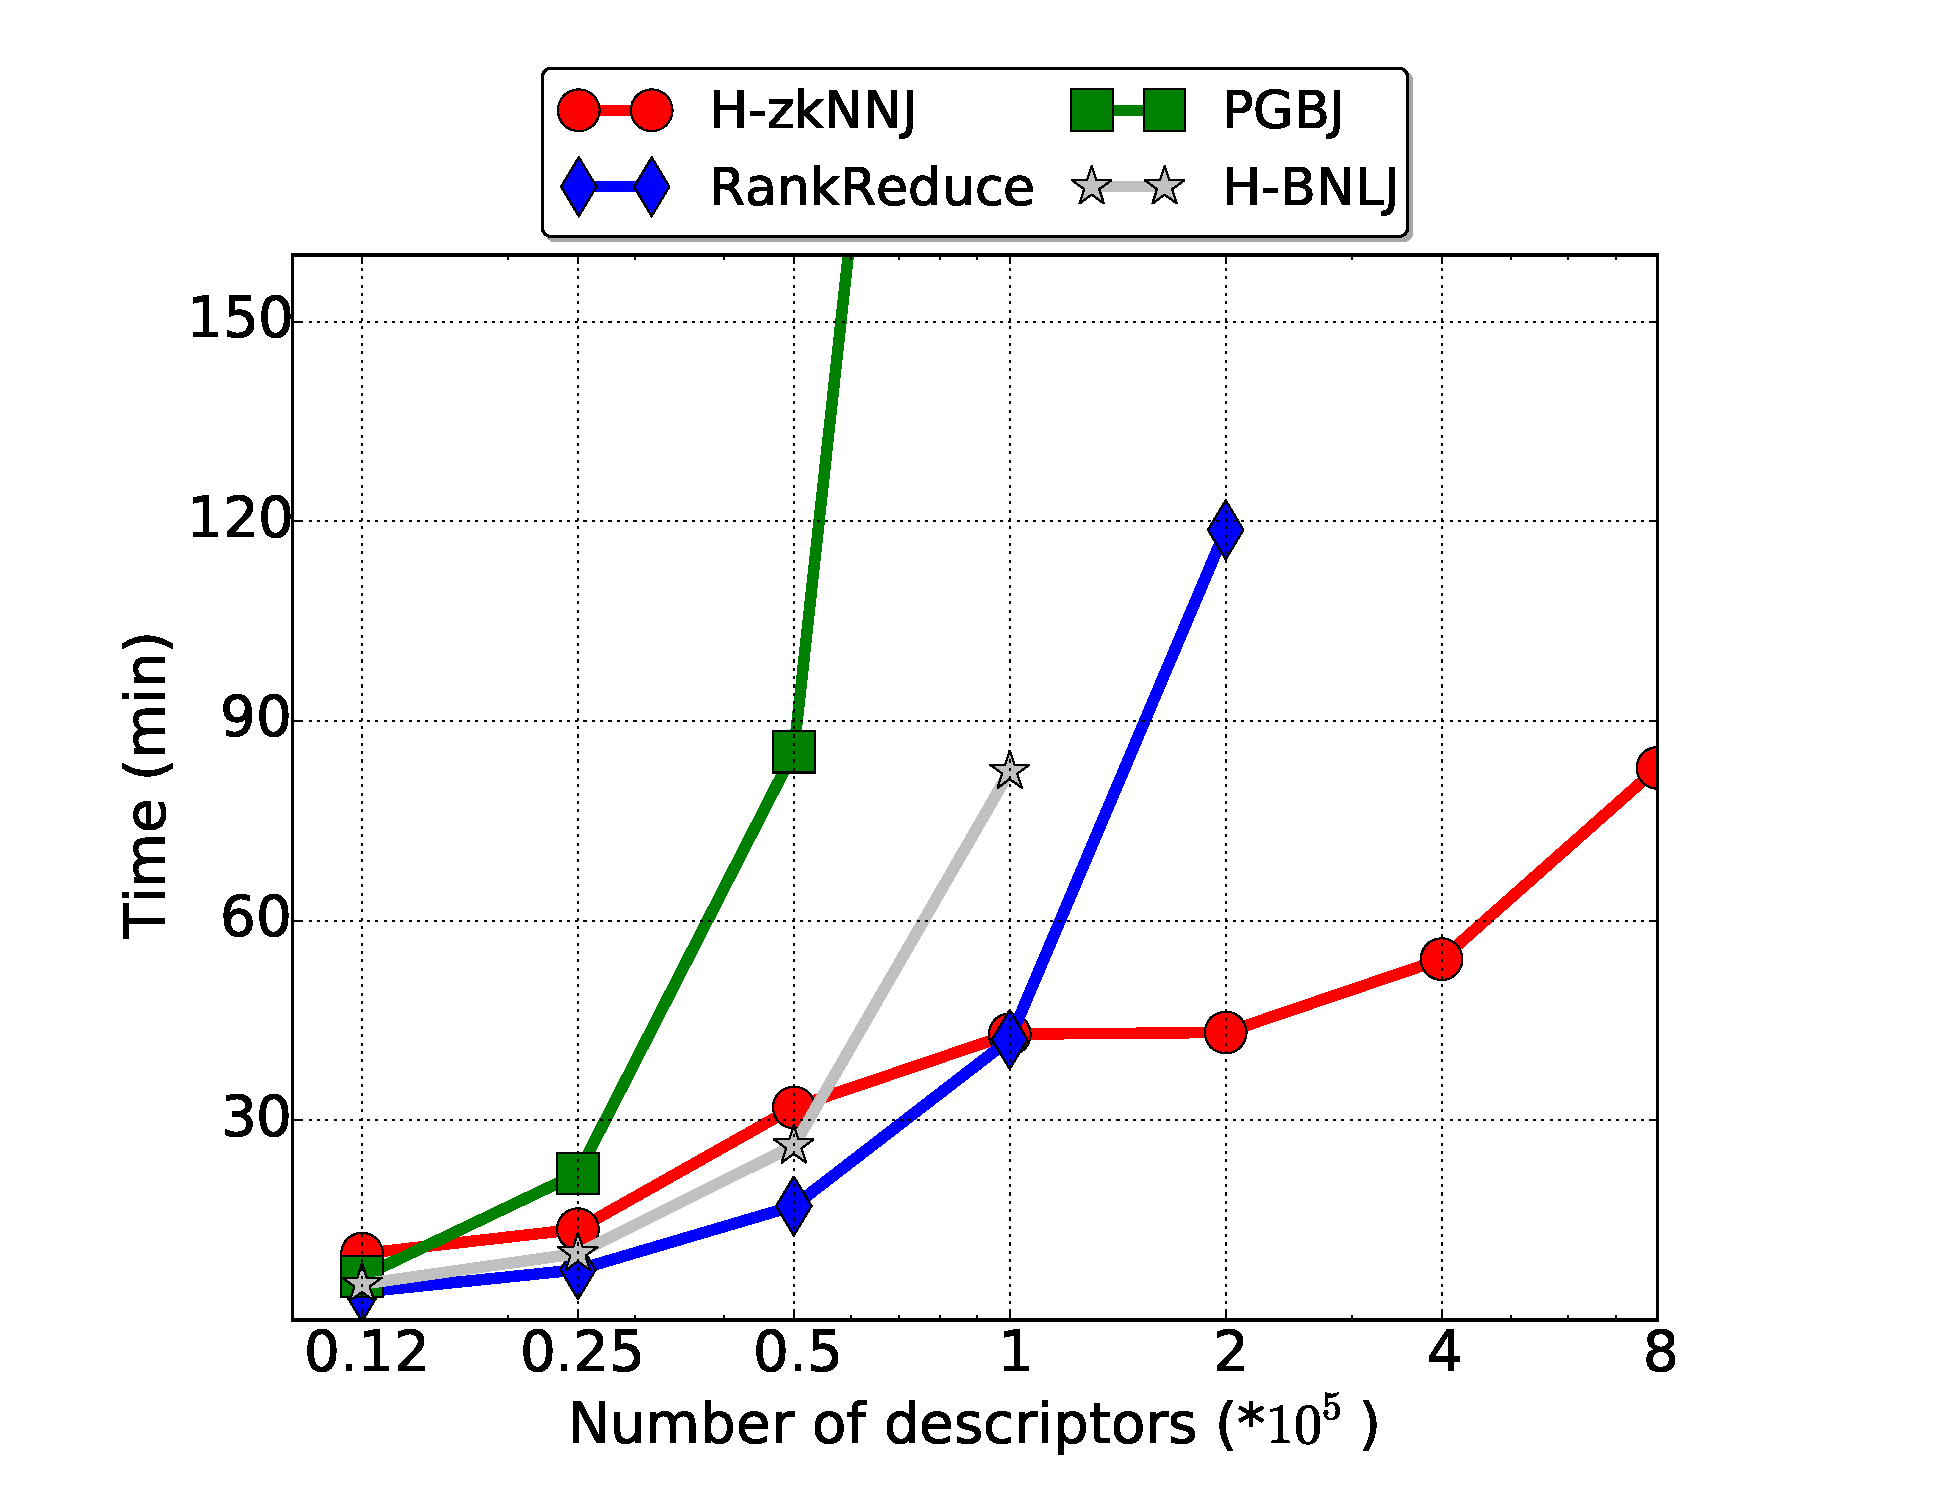
\includegraphics[width=\textwidth]{img-perf/surf/data/time.pdf}
		% }
		\caption{Time\label{fig:surf_data_time}}    
	\end{subfigure}%
	\begin{subfigure}[b]{0.35\textwidth}
		%\fbox{
		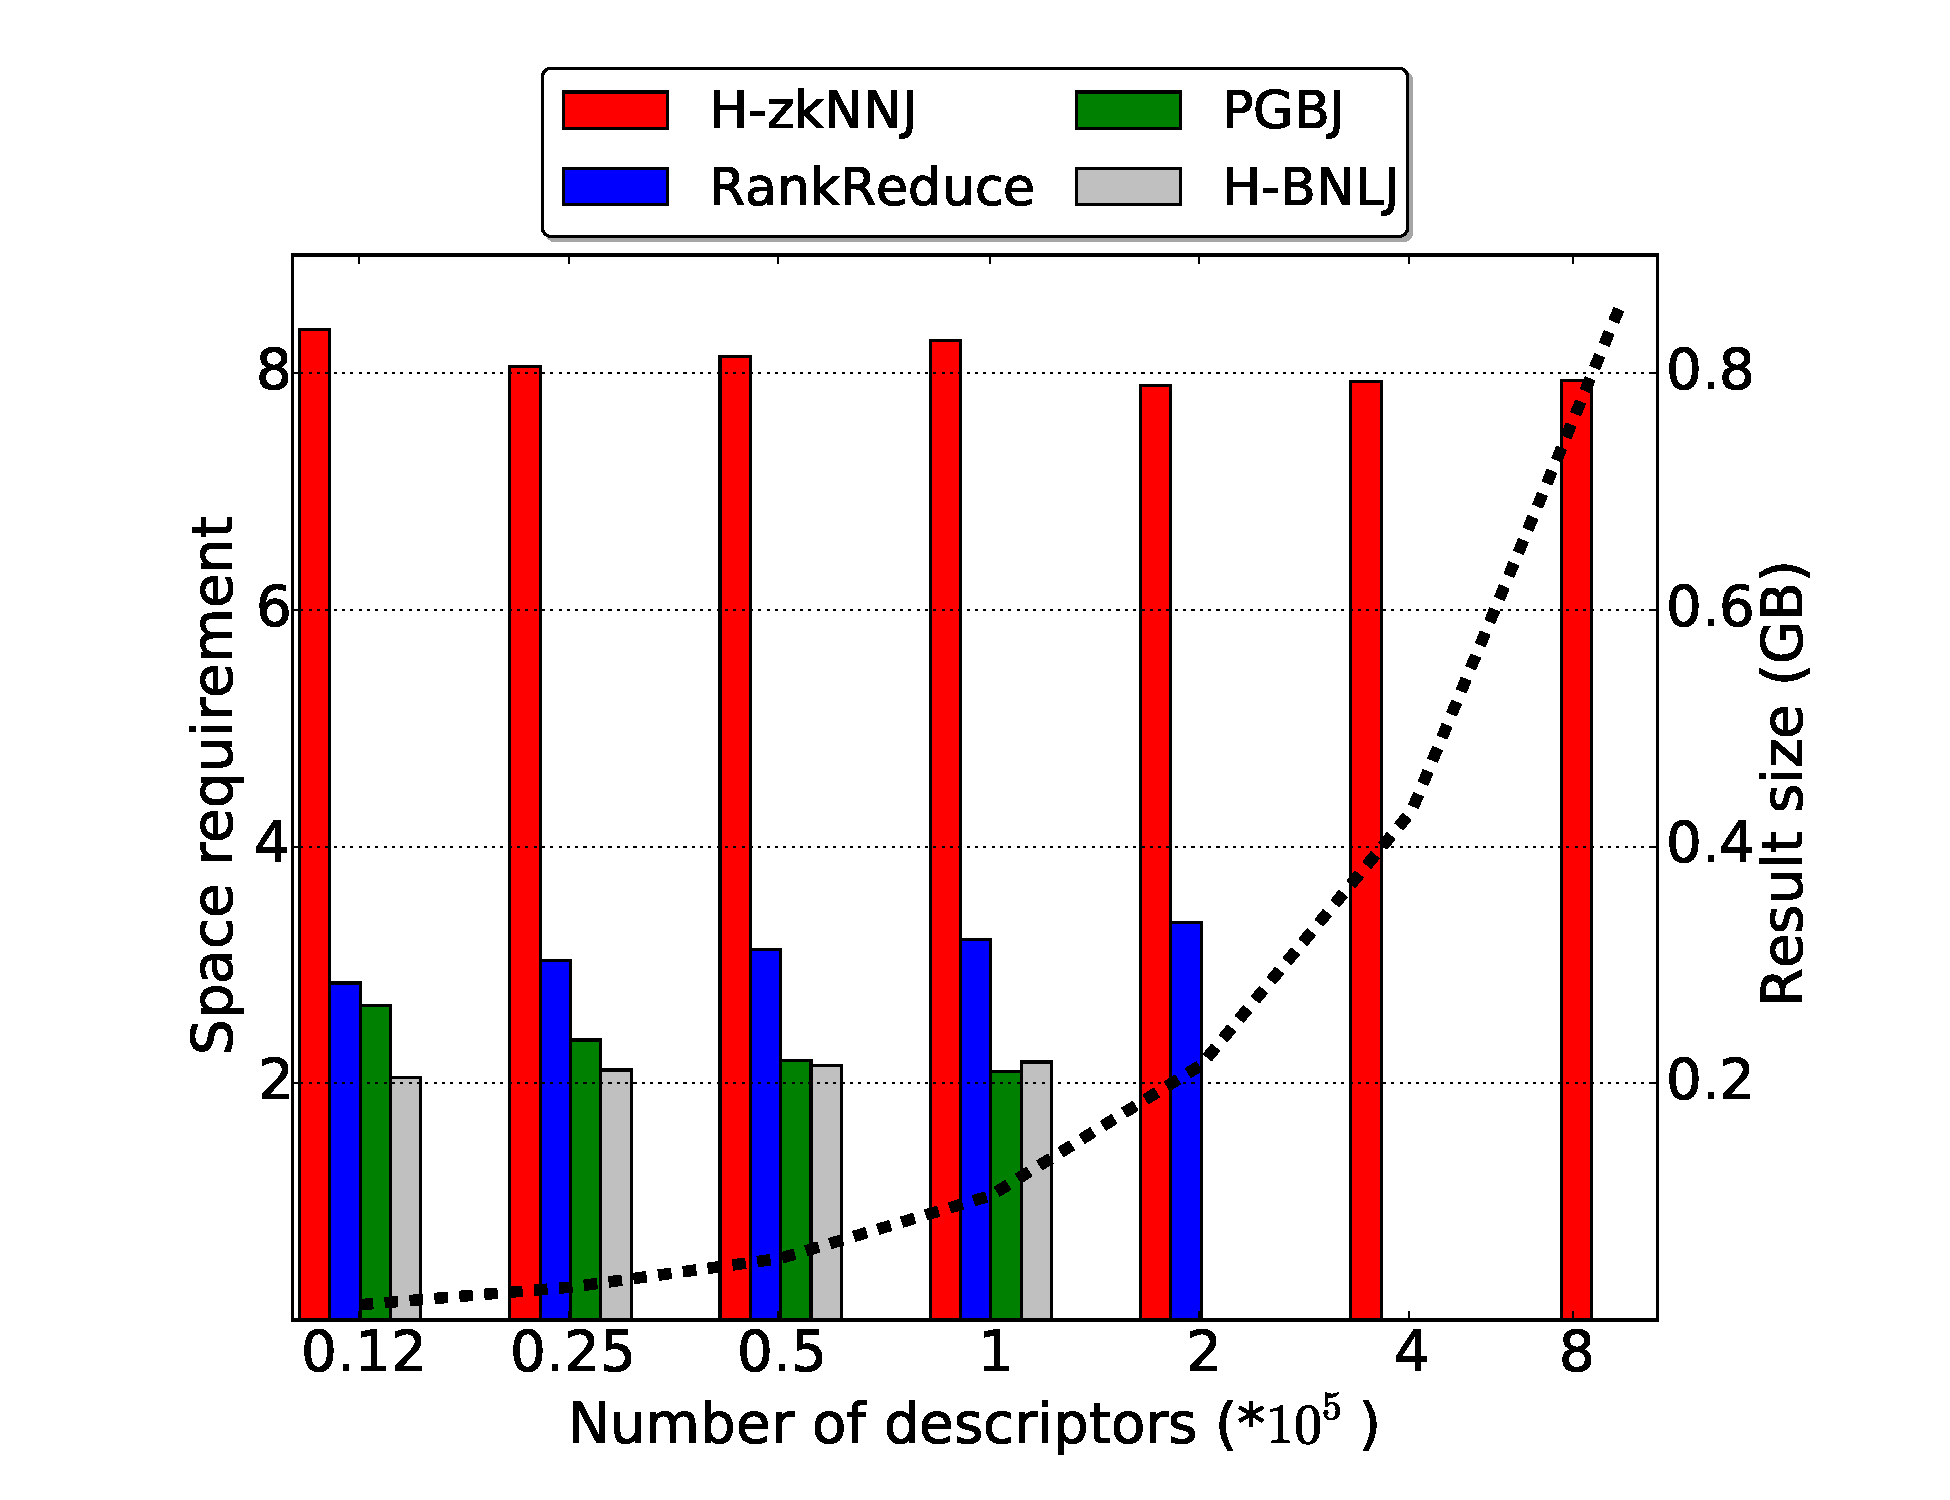
\includegraphics[width=\textwidth]{img-perf/surf/data/memory.pdf}
		%}
		\caption{Result size and Disk Usage\label{fig:surf_data_memory}}
	\end{subfigure}%       
	\begin{subfigure}[b]{0.35\textwidth}
		%\fbox{
		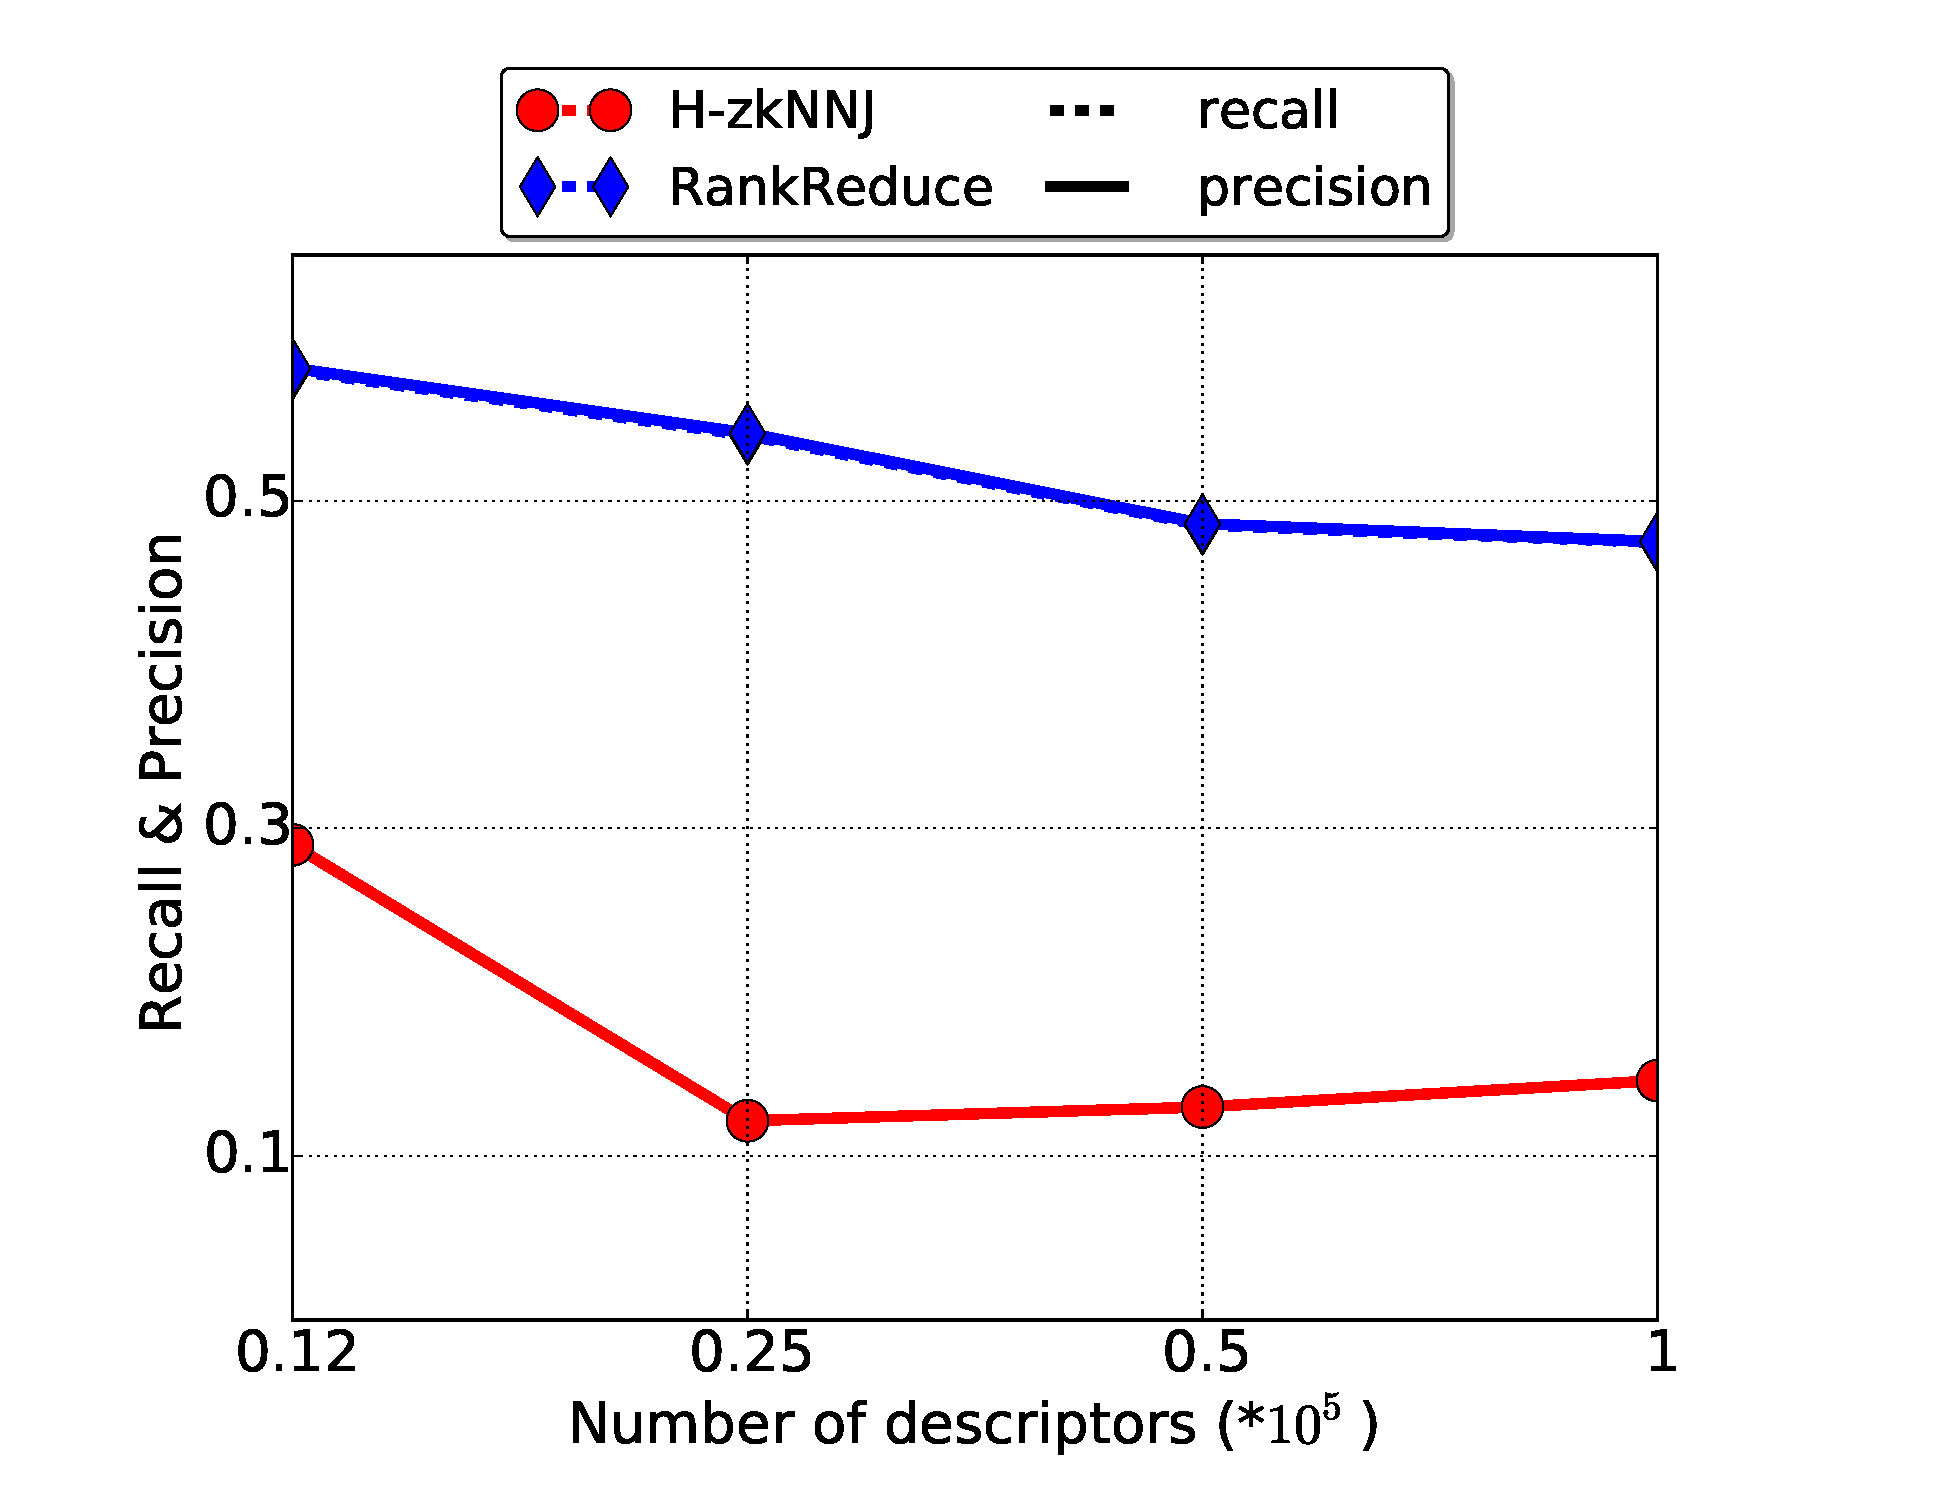
\includegraphics[width=\textwidth]{img-perf/surf/data/accuracy.pdf}
		%}
		\caption{Recall and Precision\label{fig:surf_data_acc}}        
	\end{subfigure}%  
	\caption{Surf, impact of the dataset size
		%\\ \small {Parameters : \textbf{HBNLJ} : 10partitions, \textbf{PGBJ}:$3*10^{3} pivots$, Geo grouping, kmeans 
		%sample, \textbf{RankReduce}: $L=5,M=7,W=10^{7}$ HZKNNJ : $3shift$} 
		\label{fig:surf_dataset} }
\end{figure*}

%%%% Generated by A4-ratioByK-SURF.py
\begin{figure*}[htp]
	\centering
	\begin{subfigure}[b]{0.35\textwidth}
		%\fbox{
		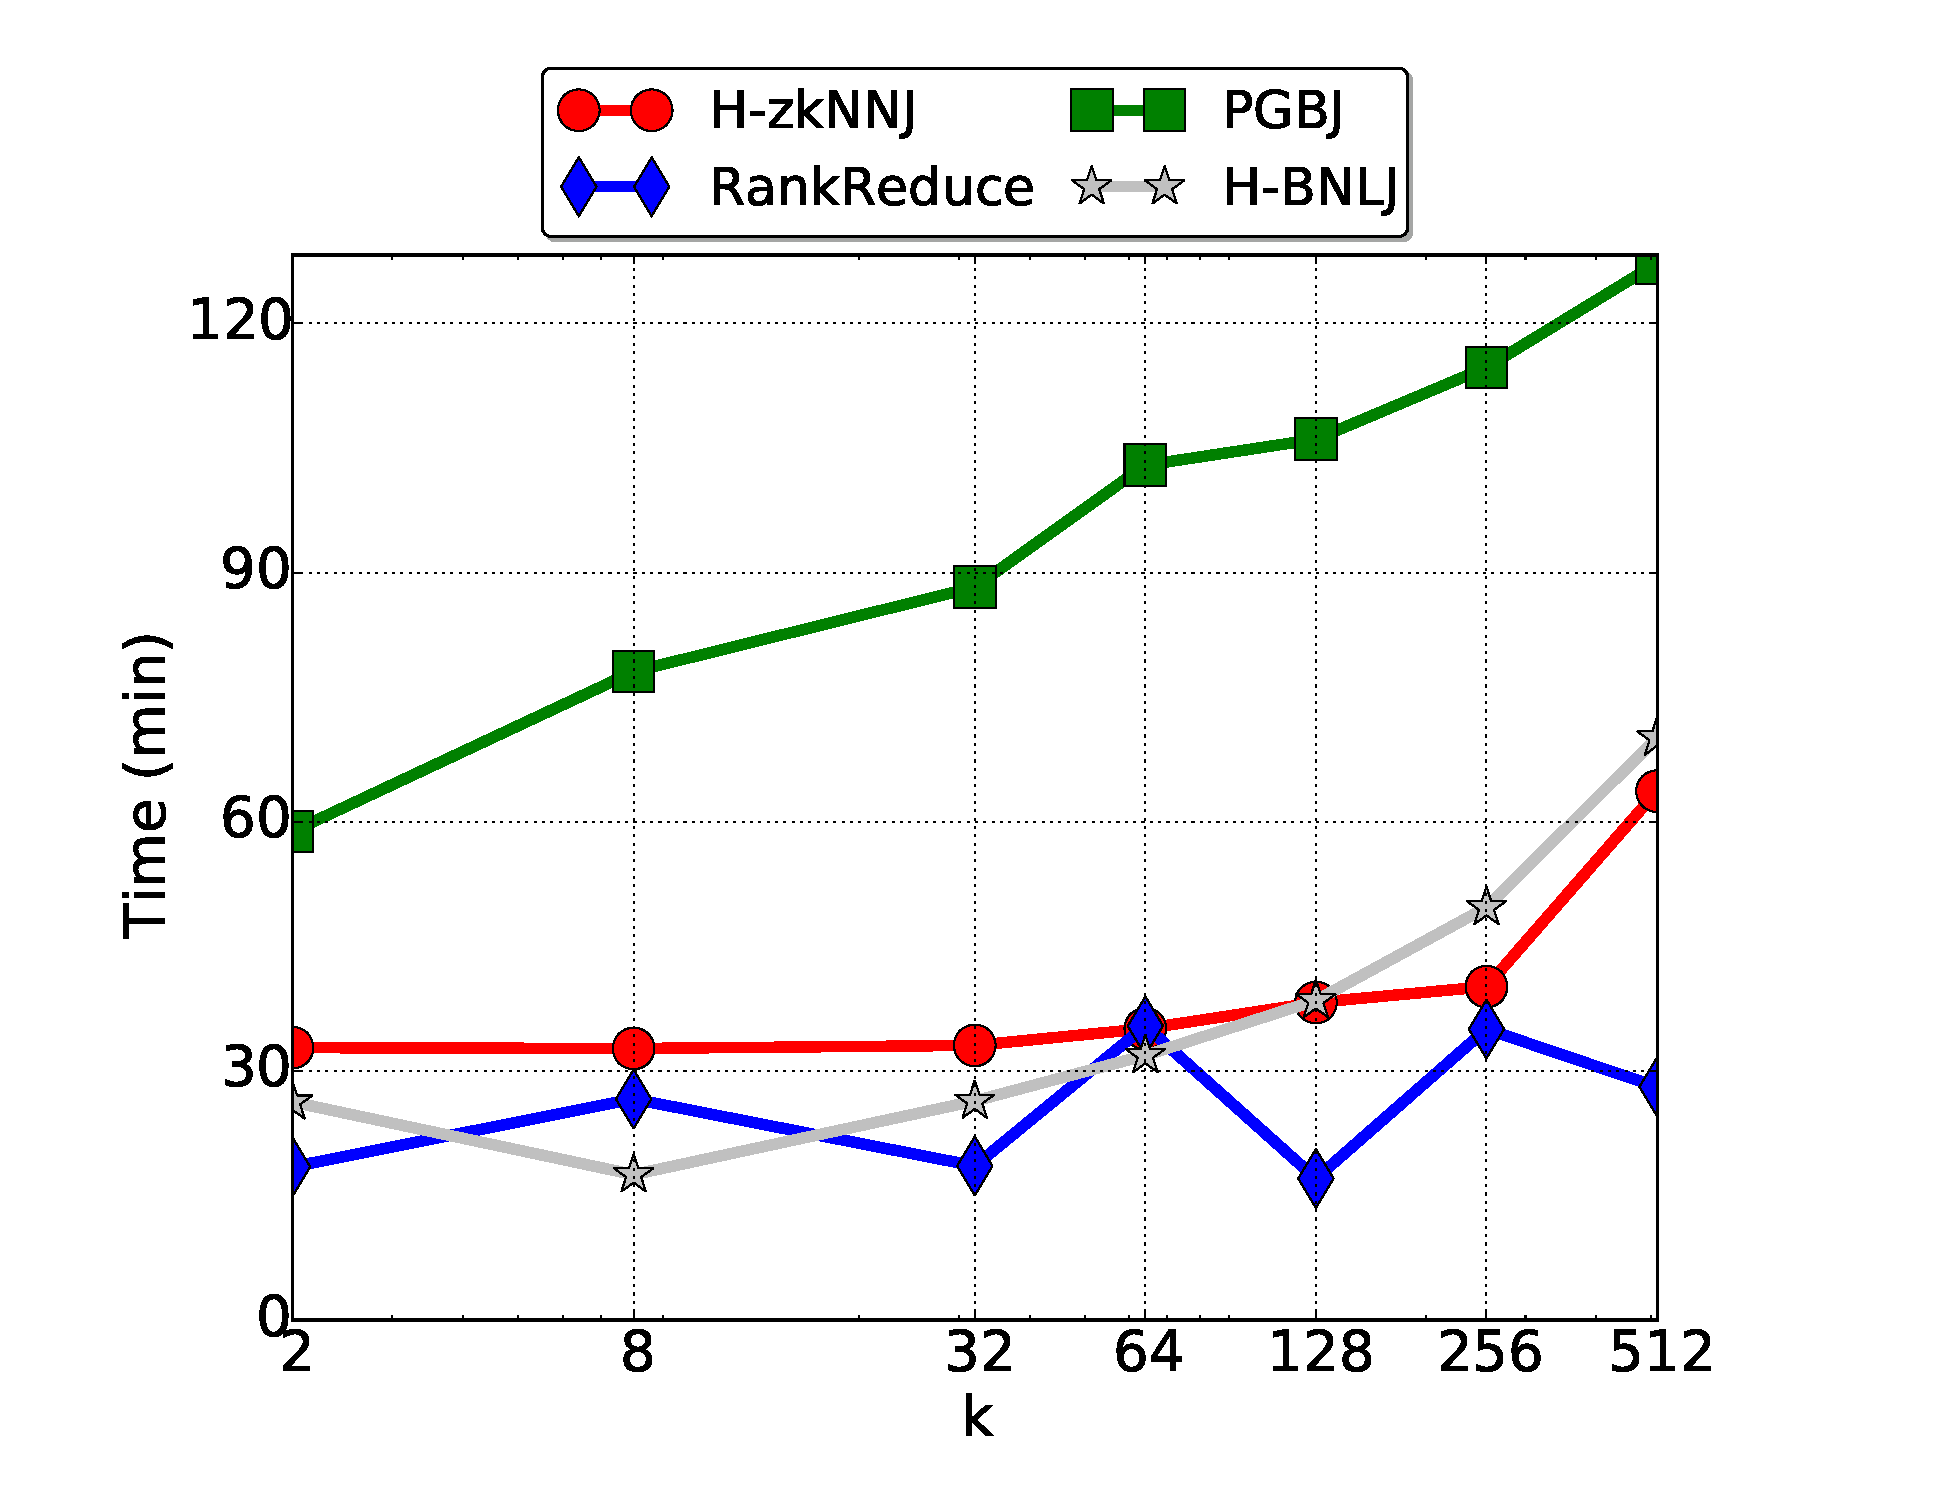
\includegraphics[width=\textwidth]{img-perf/surf/k/time.pdf} 
		%}
		\caption{Time\label{fig:surf_k_time} }
		
	\end{subfigure}%
	\begin{subfigure}[b]{0.35\textwidth}
		% \fbox{
		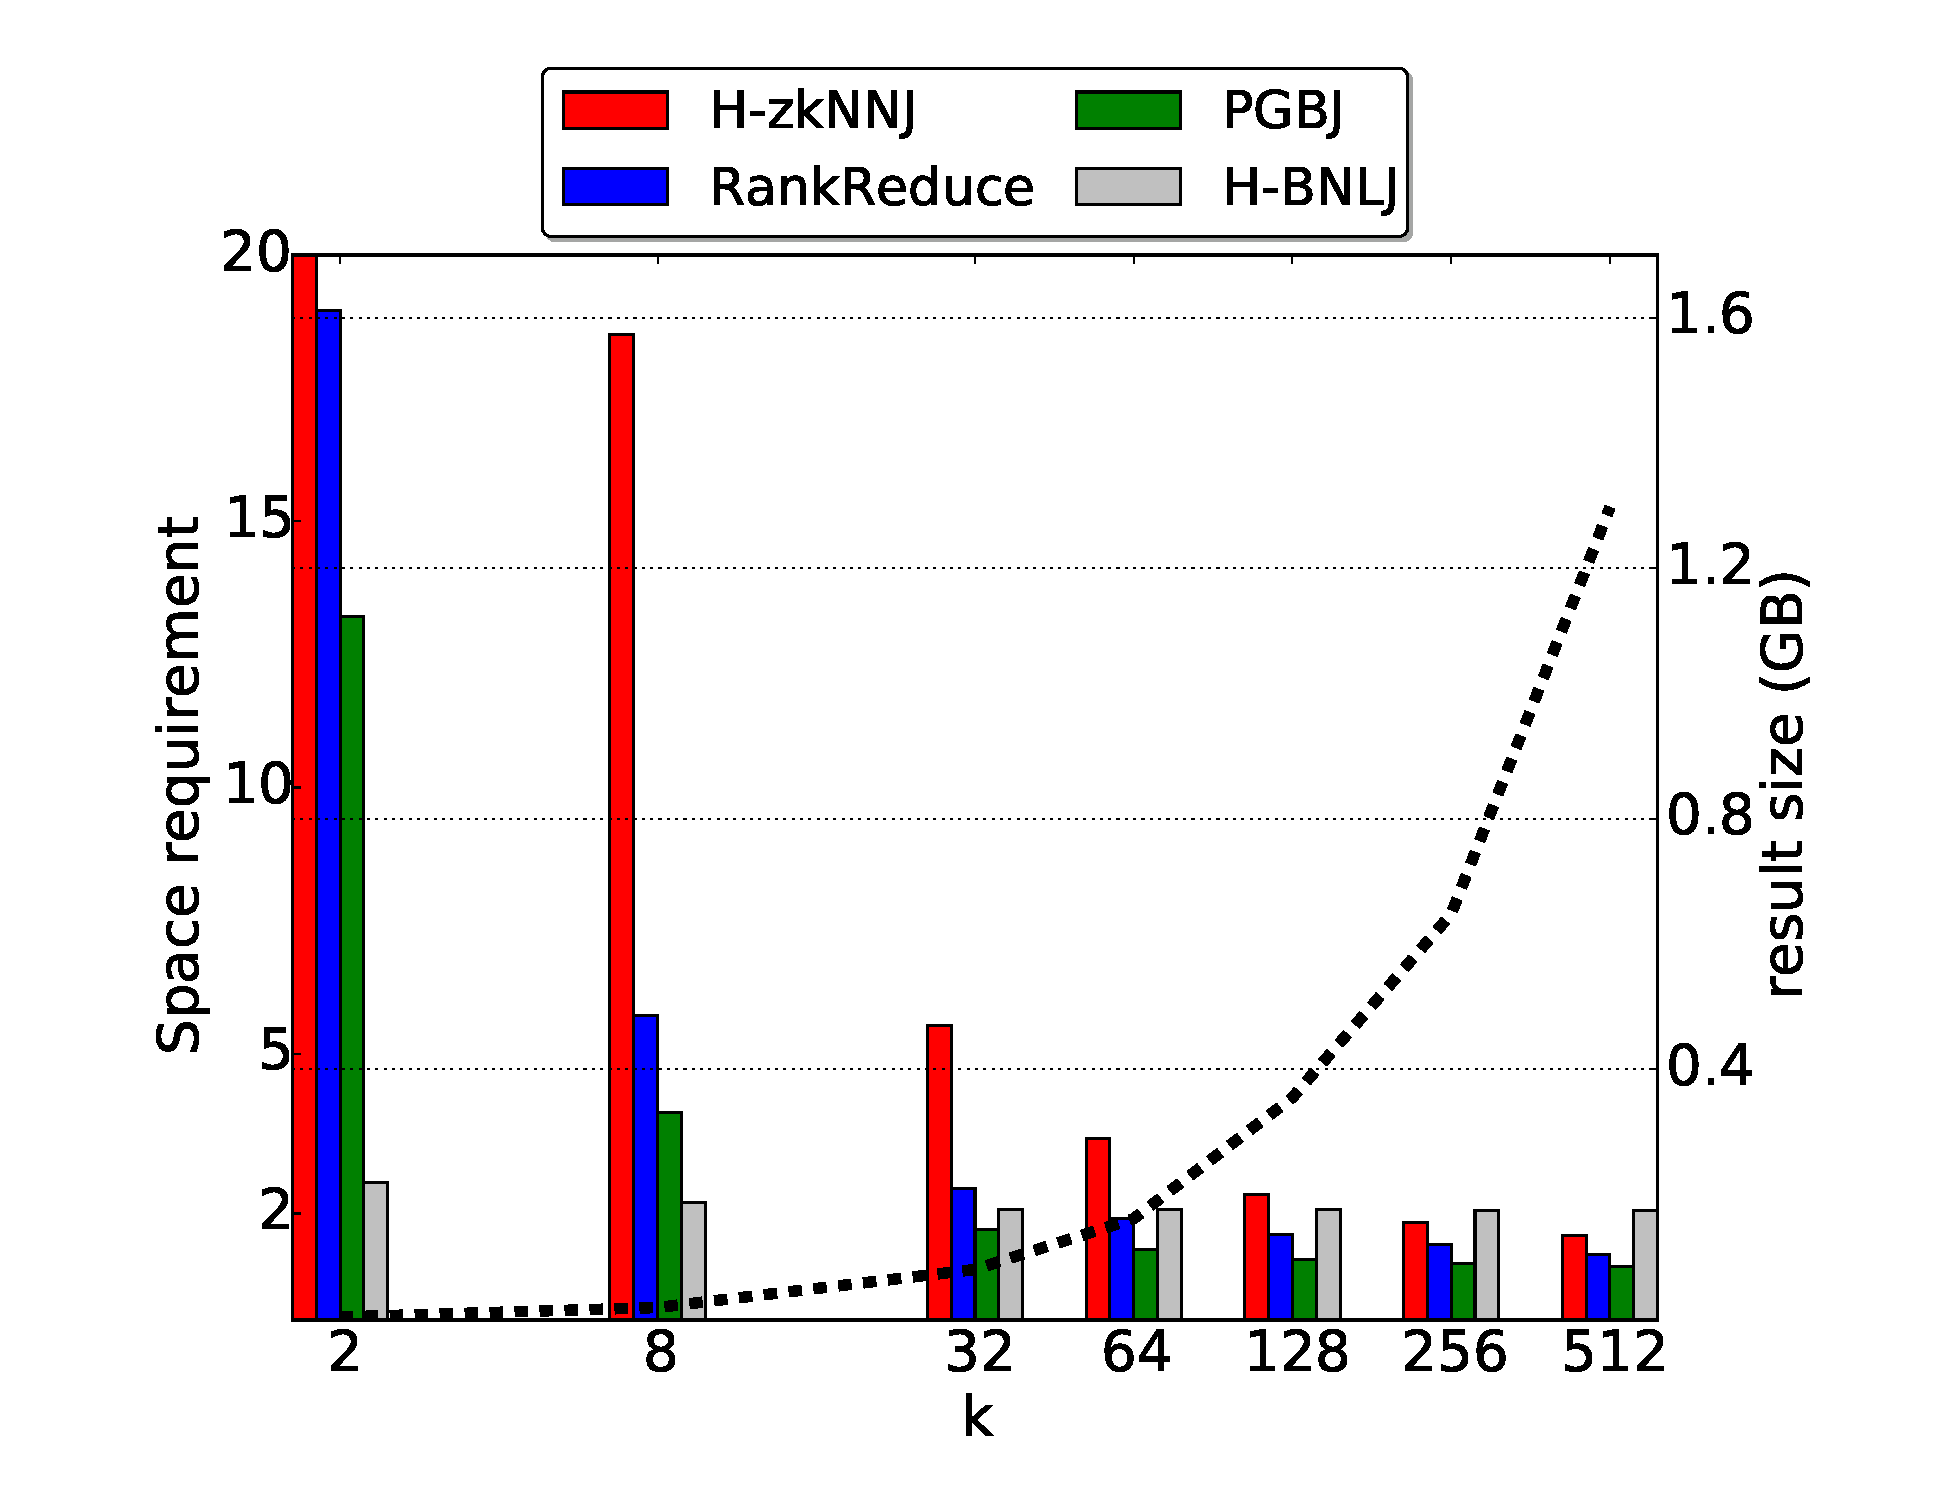
\includegraphics[width=\textwidth]{img-perf/surf/k/memory.pdf} 
		%}
		\caption{Result size and Disk Usage\label{fig:surf_k_memory}}
	\end{subfigure}%
	\begin{subfigure}[b]{0.35\textwidth}
		%\fbox{
		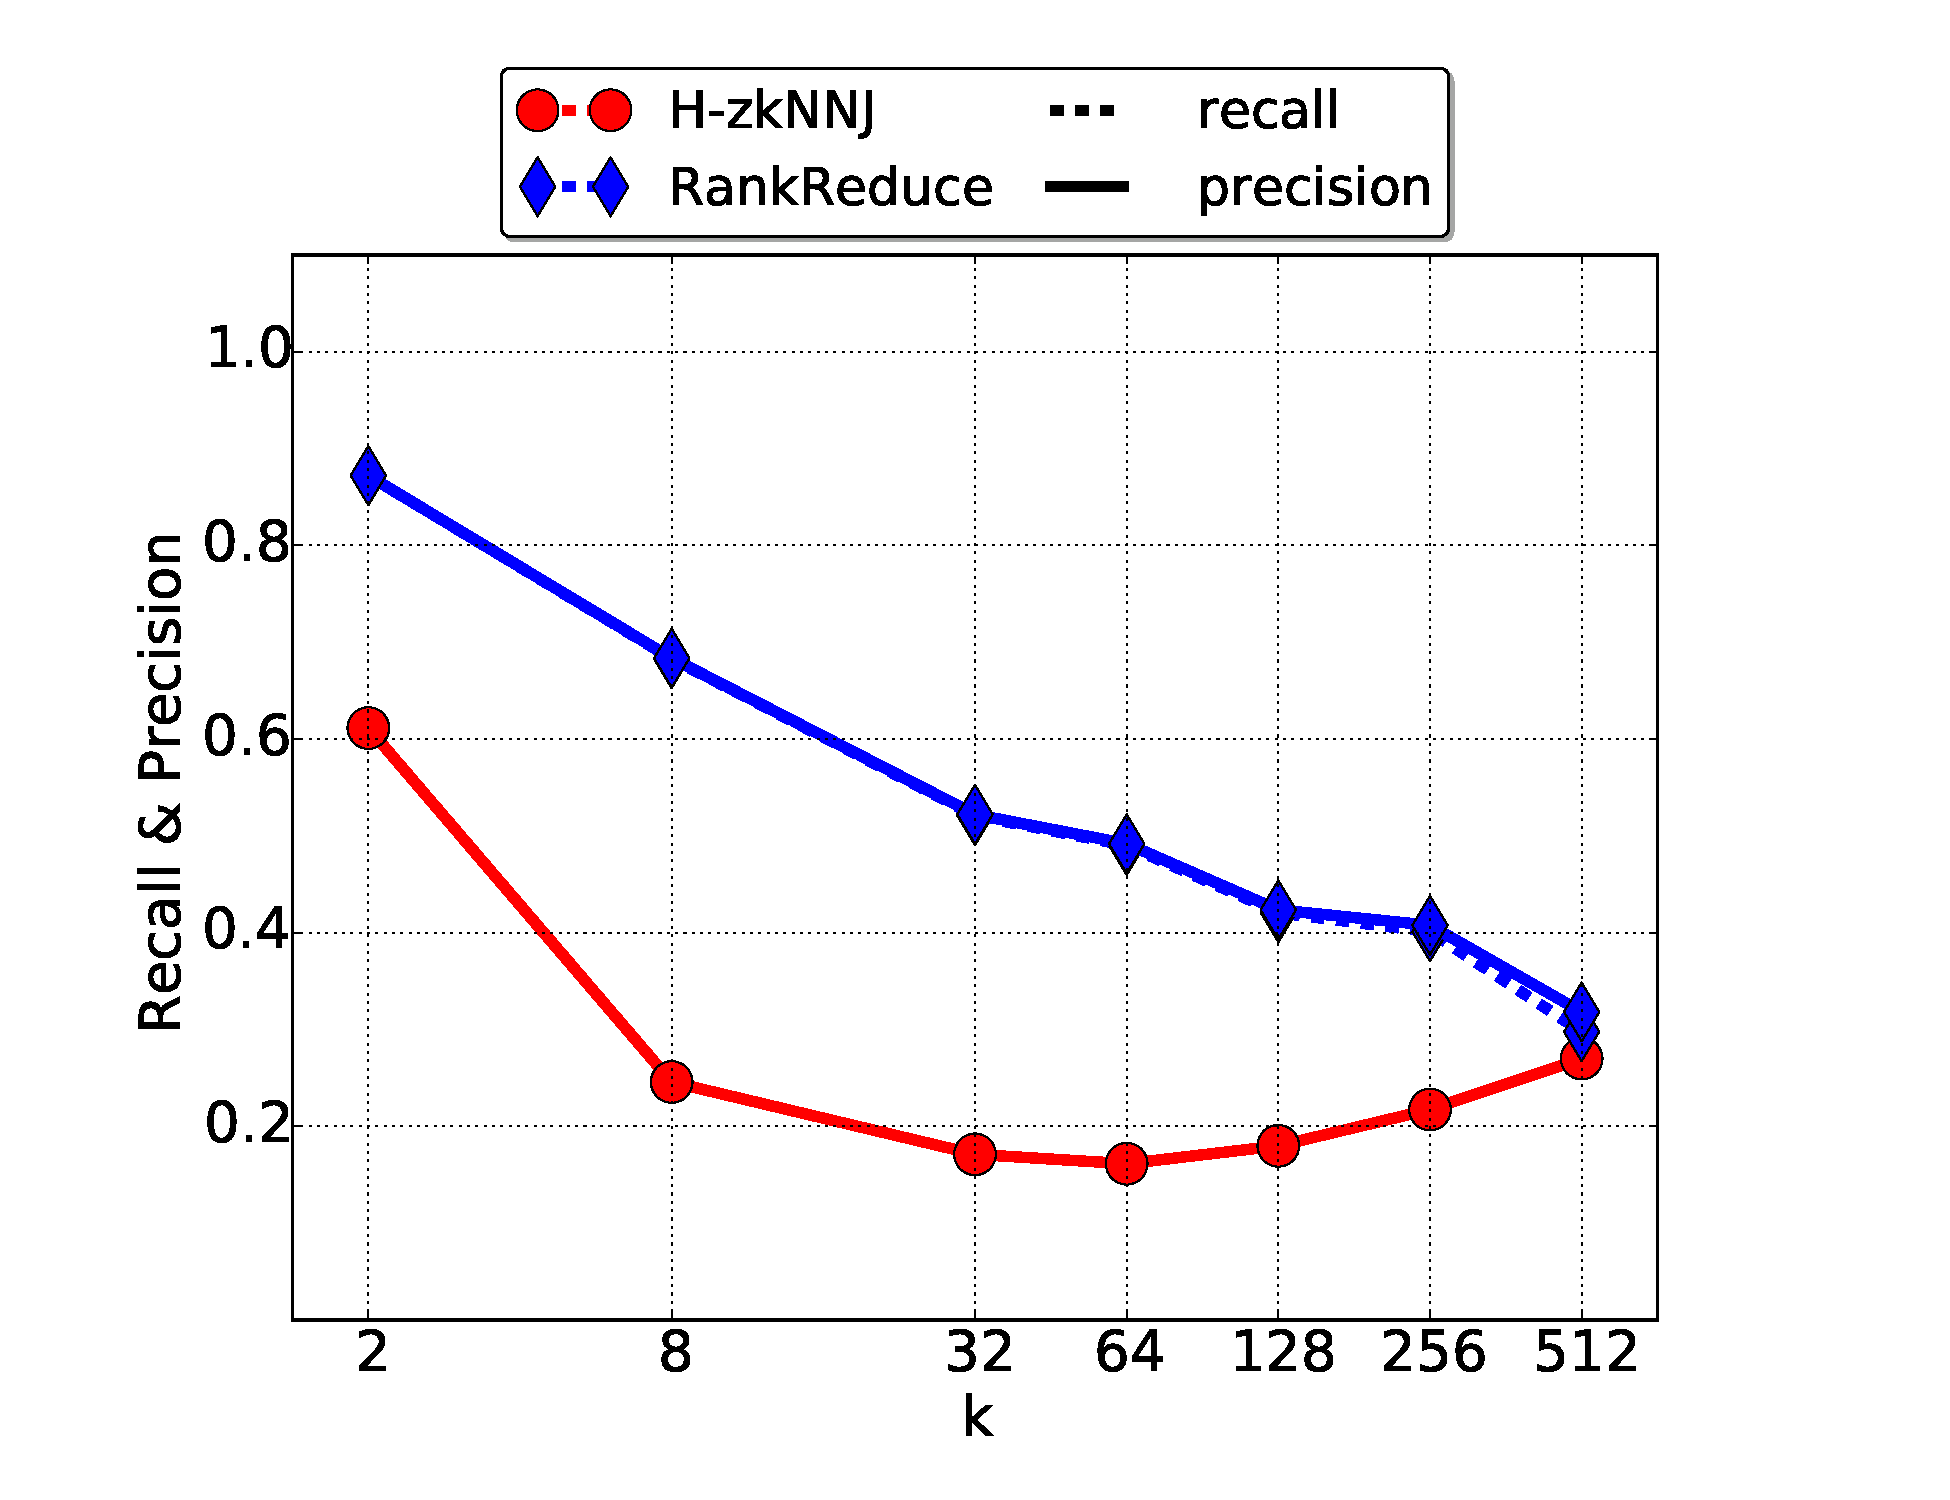
\includegraphics[width=\textwidth]{img-perf/surf/k/accuracy.pdf}
		%}
		\caption{Recall and Precision\label{fig:surf_k_acc}}
		
	\end{subfigure}%
	\caption{Surf dataset with 50k records, impact of $K$,
		%\\ \small{Parameters : \textbf{HBNLJ} : 10partition, \textbf{PGBJ}:$3*10^3 pivots$, Geo grouping, kmeans 
		%sample,\textbf{RankReduce}: $L=5,M=7,W=10^7$ HZKNNJ : $3shift$}  
		\label{fig:surf_impact_k}}
\end{figure*}


\subsubsection{Impact of input data size}

Results of experiments when varying the number of descriptors are shown in Figure~\ref{fig:surf_dataset} using a log 
scale on the x-axis. We omitted \HBK~as it could not process the data in reasonable time.
In Figure~\ref{fig:surf_data_time}, we can see that the execution time of the algorithms follows globally 
the same trend as 
with the Geo dataset, except for \VO. It is a computational intensive algorithm because the replication process implies 
calculating a lot of Euclidian distances. When in dimension 128, this part tends to dominate the overall computation 
time. Regarding disk usage (Figure~\ref{fig:surf_data_memory}), \Z~is very high because  we had to increase the number 
of shifted copies from $3$ to $5$ to 
improve the recall. Indeed, compared to the Geo dataset, it is very low (Figure~\ref{fig:surf_data_acc}). Moreover, as 
the number of descriptors 
increases, \Z~goes from 30\% to 15\% recall. As explained before, the precision was found to be equal to the recall, which means the 
algorithm always returned $k$ results. This, together with the improvement using more shifts, proves that the 
space filling curves using in \Z~are less efficient with high dimension data. 
%A solution is to 
%increase the number of shifted copies from $3$ to $5$. But the impact of time is double and no very efficient, it 
%increases just to $0.05$ the recall . \TODO{I'm confused, was the shift increased or not?}

\subsubsection{Impact of $k$}

Figure \ref{fig:surf_impact_k} shows the impact of different values of $k$ on the algorithms using a logarithmic scale 
on the x-axis.
Again, since for \HBNLJ~and \Z, the complexity of the sorting phase is dependent on $k$, we can observe a 
corresponding increase of the execution time (Figure~\ref{fig:surf_k_time}). For 
\LSH, the time varies a lot depending on $k$. This is because of the stochastic nature of the projection used in 
LSH. It can lead to buckets containing different number of elements, creating a load imbalance and some values
of $k$ naturally lead to a better load balancing. \VO~is very dependent on the value of $k$ because of the grouping 
phase. Neighboring cells are added until there are enough elements to eventually identify the $k$ nearest neighbors. 
As a consequence, a large $k$ will lead to larger group of cells and increase the computing time. 

Figure~\ref{fig:surf_k_memory} shows the effect of $k$ on disk usage. \Z~starts with a very high ratio of 74 
(not showed on the Figure) and 
quickly reduces to more acceptable values. 
 \LSH~also experiences a similar pattern to a lesser extend. As opposed to the Geo dataset, SURF 
descriptors cannot be efficiently compressed, leading to large intermediate files.

Finally, Figure~\ref{fig:surf_k_acc} shows the effect of $k$ on the recall. As $k$ increases, the recall and precision 
of \LSH~ decreases for the same reason as with the Geo dataset. Also, for large $k$, the recall becomes lower
than the precision because we get less than $k$ results. The precision of \Z~decreases but eventually shows an upward 
trend. The increased number of requested neighbors increases the number of preceding and
succeeding points copied, slightly improving the recall.
%  the number of searched $k$ reduce the probability to make 
%mistake and, 
%contrarily to \LSH, no $k$ is missing in the result (recall = precision) \TODO{Rewrite}

\subsubsection{Communication Overhead}
With the SURF dataset, we get a very different behavior than with the Geo dataset. The shuffle phase of \VO~is very 
costly (Figure~\ref{fig:surf_data_shuffle}). This is an indication of large replications incurred by the large 
dimension of the data and a poor choice of pivots. When they are too close to each other, entire cells have to be 
replicated during the grouping phase.

%%%% Generated by B00-surf.py and A4-ratioByK-SURF.py
\begin{figure*}[htp]
	\centering
	\begin{subfigure}[b]{0.48\textwidth}
		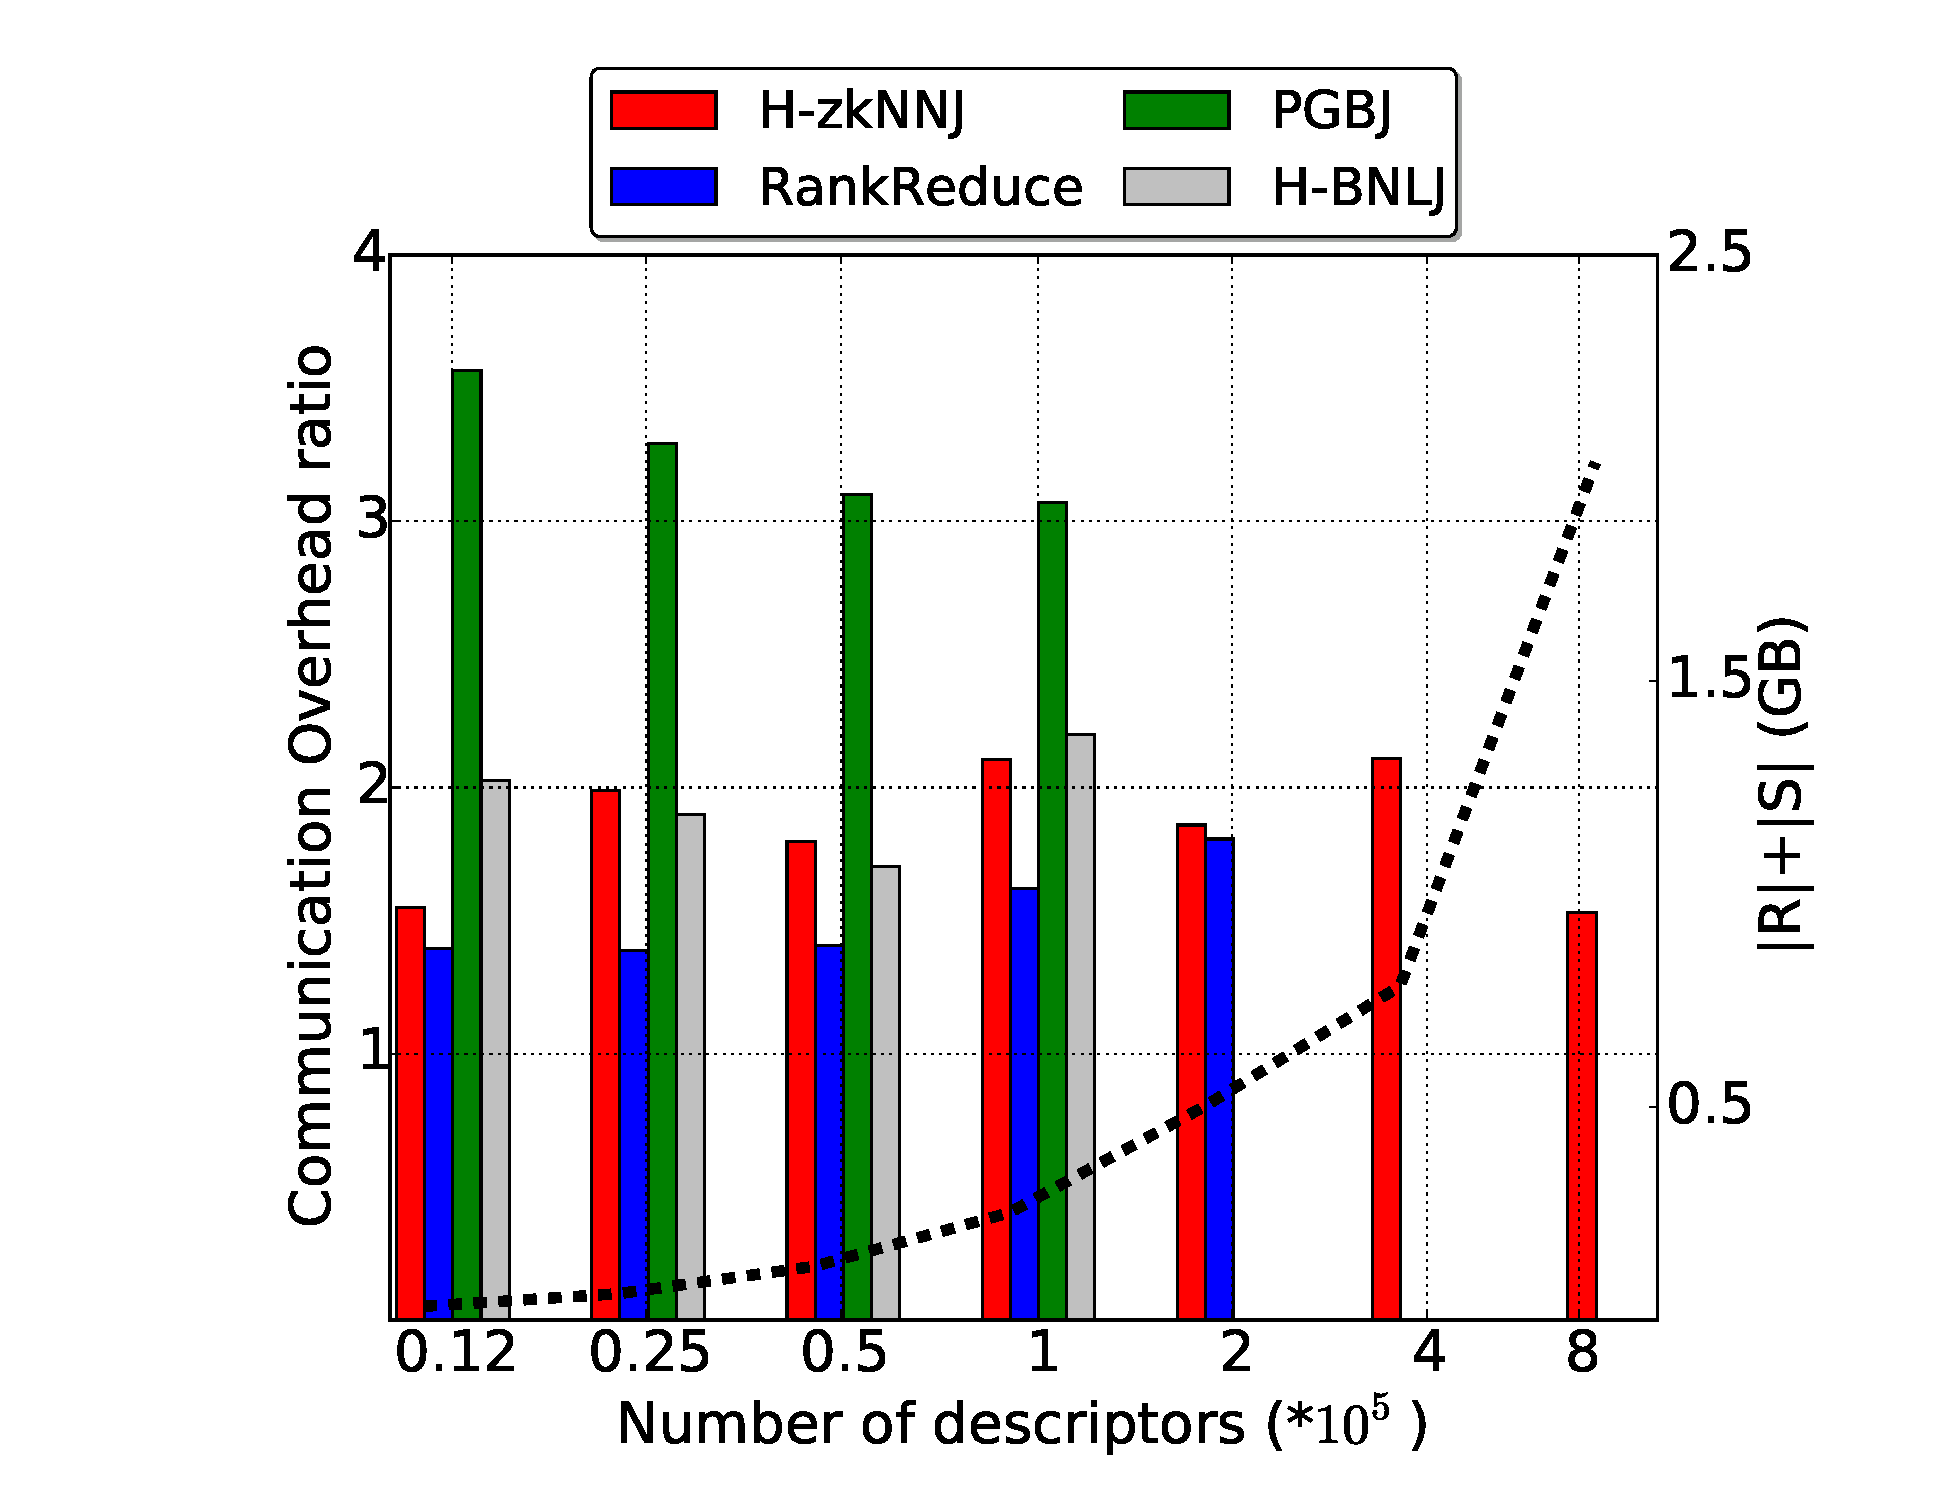
\includegraphics[width=\textwidth]{img-perf/surf/data/shuffle.pdf}
		\caption{Surf, impact of the dataset size\label{fig:surf_data_shuffle}}        
	\end{subfigure}% 
	\begin{subfigure}[b]{0.48\textwidth}
		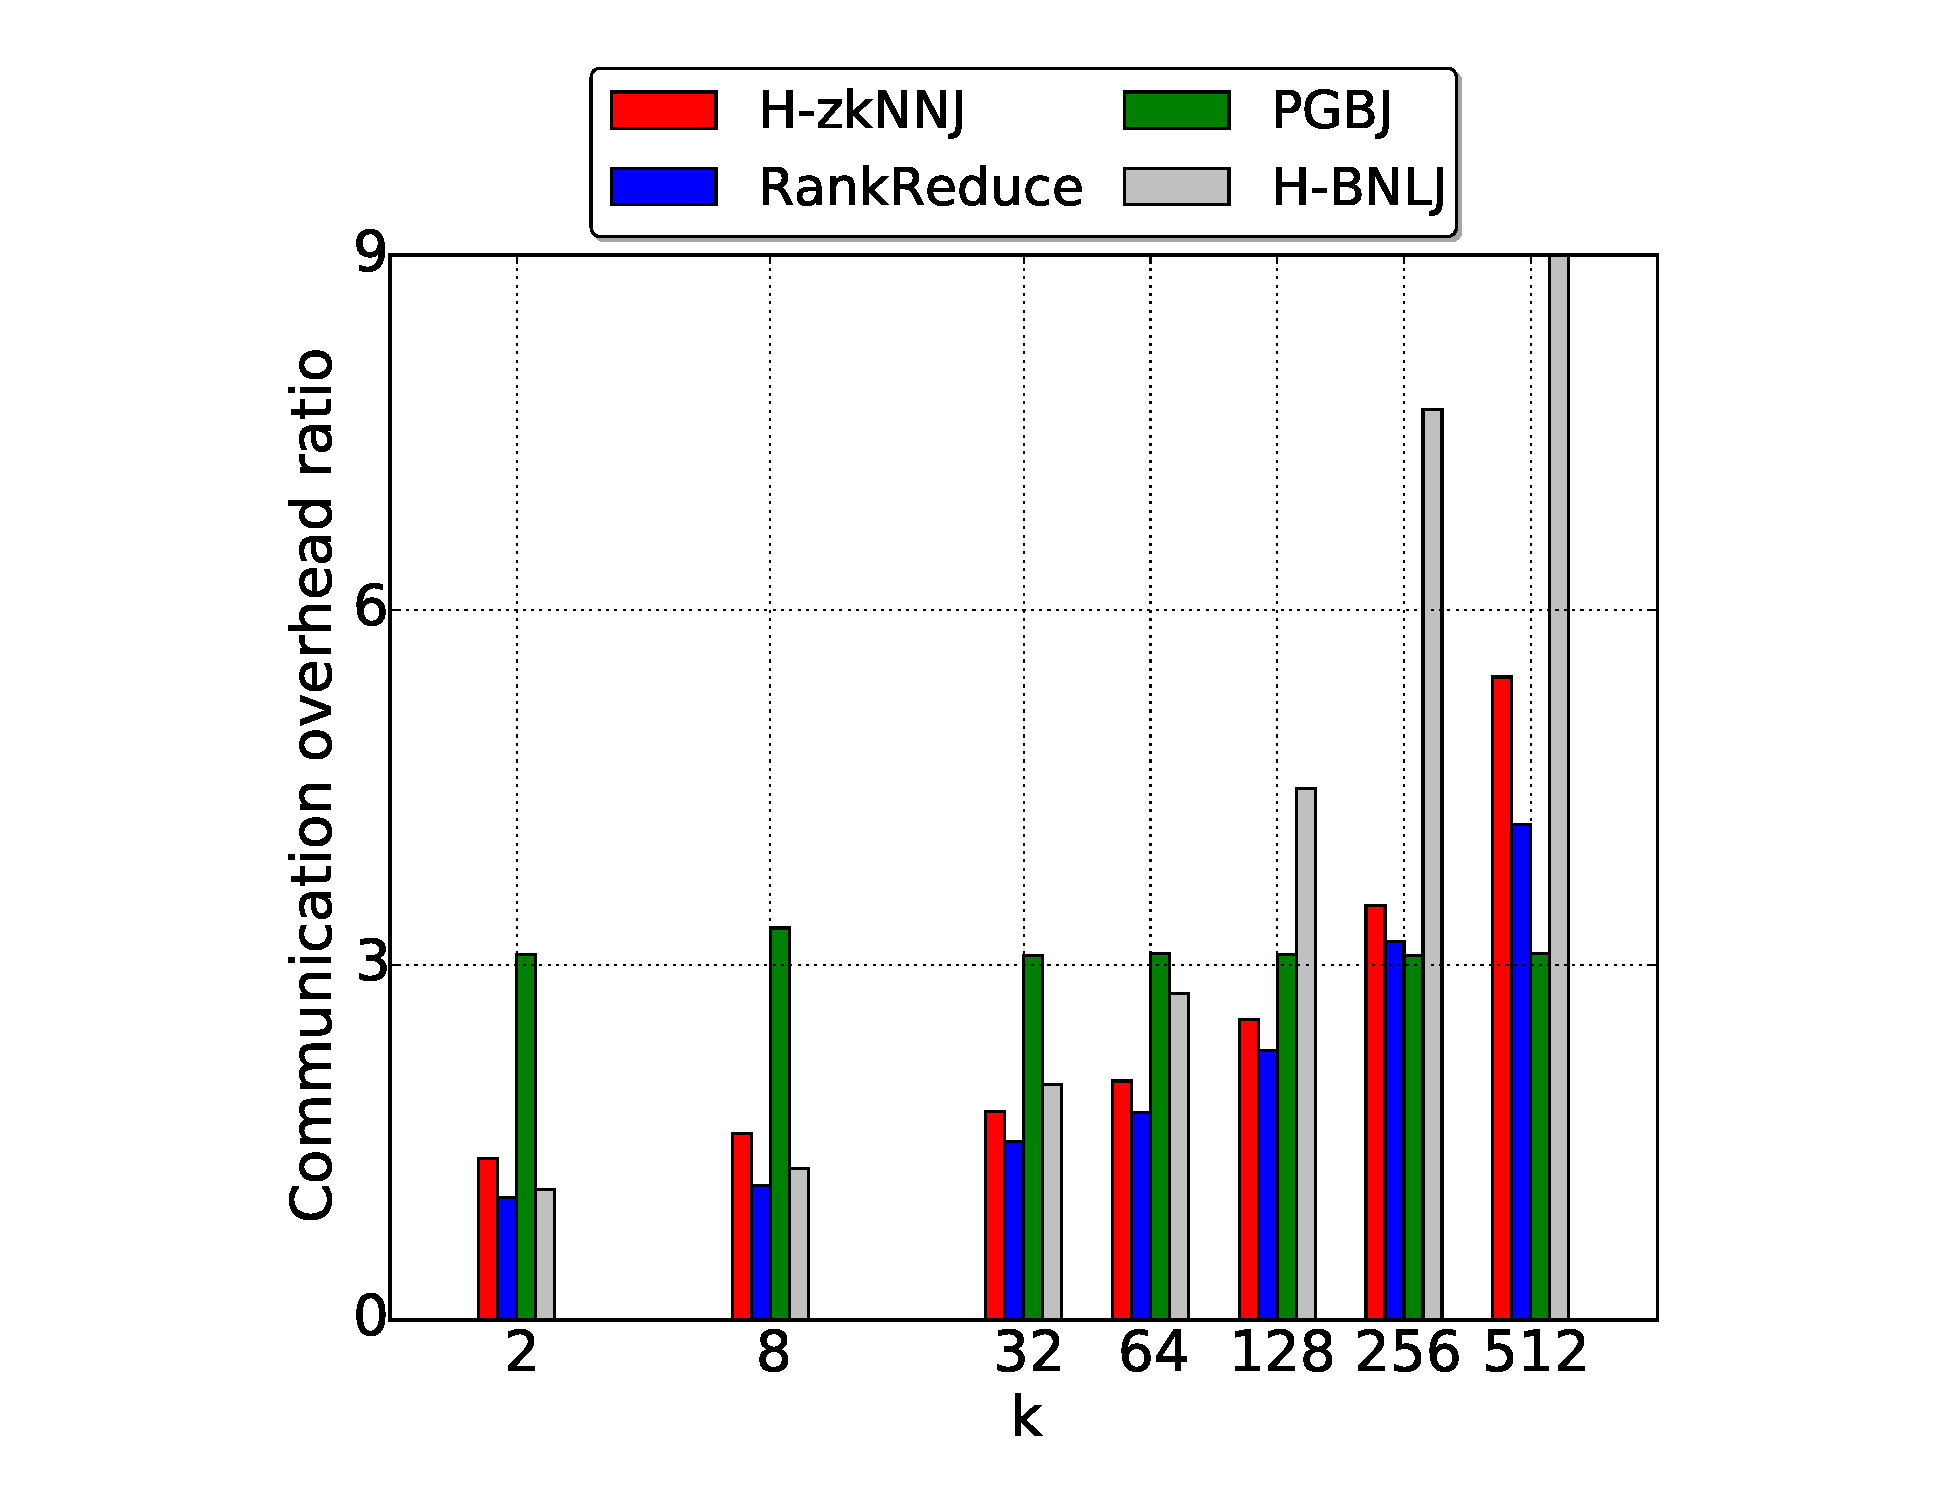
\includegraphics[width=\textwidth]{img-perf/surf/k/shuffle.pdf} 
		\caption{Surf dataset with 50k records, impact of $K$,\label{fig:surf_k_shuffle}}
	\end{subfigure}%
	\caption{Communication overhead for the Surf dataset}      
\end{figure*}


For \LSH~the shuffle is decreased but stay important, essentially because of the replication factor of $5$. Finally,
the shifts of original data in \Z~lead to a large communication overhead. 


Considering now $k$, we have the same behavior we observed with the Geo dataset. The only difference is \VO~which now exhibits a
large communication overhead (Figure~\ref{fig:surf_k_shuffle}). This is again because of the choice of pivots and 
the grouping of the cells. However, this overhead remains constant, irrespective of $k$. 